\documentclass[10pt]{beamer}

\usetheme[progressbar=frametitle]{metropolis}
\usepackage{appendixnumberbeamer}
\usepackage[utf8]{inputenc}
\usepackage{booktabs}
\usepackage[scale=2]{ccicons}
\usepackage{xcolor}
\usepackage{pgfplots}
\usepgfplotslibrary{dateplot}
\usepackage{xspace}


\usepackage{listings}


% Emulate markdown's light grey background for monospace.
\usepackage{soul}
\definecolor{Light}{gray}{.96}
\sethlcolor{Light}
\let\OldTexttt\texttt
\renewcommand{\texttt}[1]{\OldTexttt{\hl{#1}}}% will affect all \texttt


%  Use knitr's colorscheme.
\definecolor{fgcolor}{rgb}{0.345, 0.345, 0.345}
\definecolor{hlnum}{rgb}{0.686,0.059,0.569}
\definecolor{hlstr}{rgb}{0.192,0.494,0.8}
\definecolor{hlcom}{rgb}{0.678,0.584,0.686}
\definecolor{hlopt}{rgb}{0,0,0}
\definecolor{hlstd}{rgb}{0.345,0.345,0.345}
\definecolor{hlkwa}{rgb}{0.161,0.373,0.58}
\definecolor{hlkwb}{rgb}{0.69,0.353,0.396}
\definecolor{hlkwc}{rgb}{0.333,0.667,0.333}
\definecolor{hlkwd}{rgb}{0.737,0.353,0.396}
\definecolor{shadecolor}{rgb}{0.969, 0.969, 0.969}

\lstset{
  backgroundcolor=\color{shadecolor},
  basicstyle=\color{hlstd}\ttfamily\footnotesize,
  breakatwhitespace=false,
  %breaklines=true,
  captionpos=b,
  commentstyle=\color{hlcom},
  deletekeywords={...},
  escapeinside={\%*}{*)},
  extendedchars=true,
  frame=lines,
  keepspaces=true,
  keywordstyle=\color{hlkwb},
  morekeywords={*,...},
  numbers=left,
  numbersep=5pt,
  numberstyle=\tiny\color{hlstd},
  rulecolor=\color{hlstd},
  showspaces=false,
  showstringspaces=false,
  showtabs=false,
  stepnumber=1,
  stringstyle=\color{hlstr},
  tabsize=2,
  title=\lstname
}

\newcommand{\themename}{\textbf{\textsc{metropolis}}\xspace}

\title{KodeKlubben 2.0}
\subtitle{Øvelsesgang 1}
% \date{\today}
\date{\today}
\author{Kristian Urup Olesen Larsen, Jakob Jul Elben}
\institute{Økonomisk Institut, KU}
% \titlegraphic{\hfill\includegraphics[height=1.5cm]{logo.pdf}}

\begin{document}

\maketitle

\begin{frame}[fragile]{Velkommen!}
Hvem er vi?
\begin{itemize}
  \item Økonomistuderende
  \item RA's på Økonomisk Institut
  \item Arbejder typisk i Python, R, STATA eller SAS
\end{itemize}
Hvem er i?
% \begin{itemize}
%   \item Det er sådan set ligemeget, vi skal bare have det sjovt og lære noget \textit{data science}.
% \end{itemize}
\end{frame}

\begin{frame}[fragile]{Setup}
  Alt materiale ligger på GitHub
\begin{itemize}
  \item Åben \href{https://github.com/Kristianuruplarsen/kodeklubben}{https://github.com/Kristianuruplarsen/kodeklubben}
  \item Klik på knappen \textit{Clone or download} og på \textit{Download ZIP}
\end{itemize}

\begin{figure}
  \center
  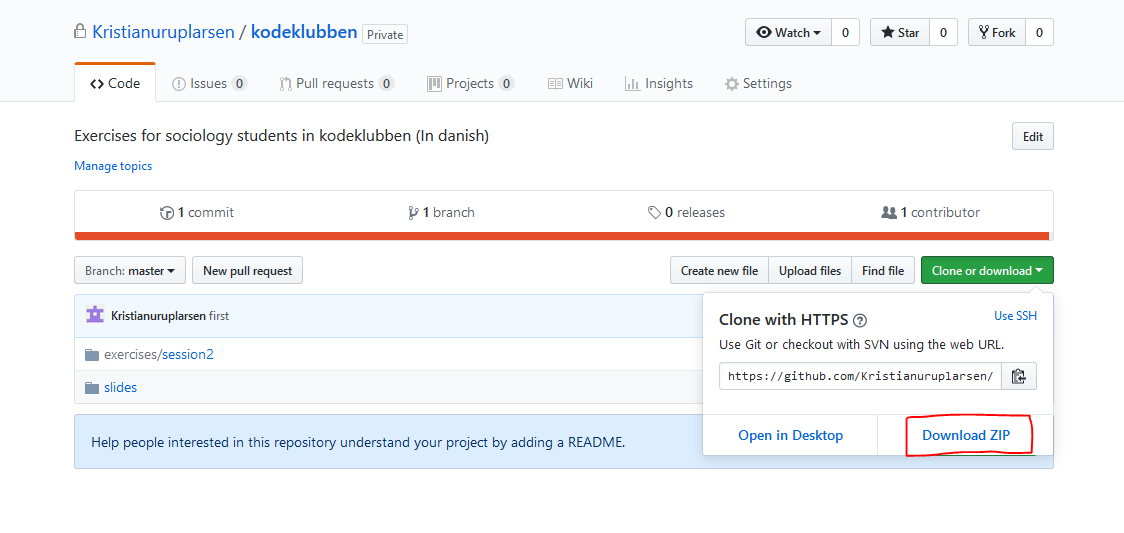
\includegraphics[width=\textwidth]{figs/setup.PNG}
\end{figure}
\end{frame}


\begin{frame}[fragile]{Hvad skal vi lave?}
\begin{itemize}
  \item<1-> Hvad mener (folketings)partierne egentligt? Gid vi kunne spørge dem...
  \item<2-> DR's kandidattest fra KV17 er stadig online!
  \item<3-> Alle kandidaternes svar er ``frit'' tilgængelige.
  \item[]
  \item[]<4-> Kort note om formattet:
  \item<4-> Vi har slides der viser hvordan i kan løse alle spørgsmålene,
  \item[]<5-> men den bedste vej frem er \textit{learning by doing}
  \item<6-> 1) Læs dokumentation 2) spørg en sidemakker 3) google det (stackoverflow har som regel løsningen) 4) spørg os.
\end{itemize}


\end{frame}

\begin{frame}[fragile]{Projektet}
Op til KV17 lavede DR en \href{https://www.dr.dk/nyheder/politik/kv17/kandidat-testen}{kandidattest}. Alle kandidaterne har selvfølgelig svaret på spørgsmålene. De svar vil vi gerne have.

Denne gang:
\begin{itemize}
  \item Download data fra DR
  \begin{itemize}
    \item internet-hacks
    \item Interagere med nettet gennem python
  \end{itemize}
  \item Rens datasættet og gør klar til alt det sjove
  \begin{itemize}
    \item jonglere med data og formatter
  \end{itemize}
\end{itemize}

Næste gang:
\begin{itemize}
  \item Alt det sjove.
  \begin{itemize}
    \item \textit{Dimensionality reduction}
    \item Interaktive plot
  \end{itemize}
\end{itemize}
\end{frame}





\section{Øvelser}


\begin{frame}[fragile]{Opgave 1.1}
  Det link i leder efter er:
  \begin{centering}\textit{
  \href{'https://www.dr.dk/tjenester/kv17-candidateapi/api/constituency/all'}{https://www.dr.dk/tjenester/kv17-candidateapi/api/constituency/all}}
  \end{centering}
  Prøv at åbne linket i en browser!
\end{frame}

\begin{frame}[fragile]{Opgave 1.2}
  \begin{itemize}
    \item Hvis ikke i har installeret \texttt{requests} er det en god ide at gøre det nu
    \item Google:
    \begin{itemize}
      \item ``python requests get link''
      \item ``python requests json''
    \end{itemize}
  \end{itemize}

  \begin{lstlisting}[language=python]
import requests

url = #[FILL IN]

response = requests.get(url)
kommuner = response.json()
  \end{lstlisting}
\end{frame}

\begin{frame}[fragile]{Opgave 1.3}
  \begin{itemize}
    \item Kig i den json fil i har downloadet - hvordan er den struktureret?

    \item I kan hente alle slugs med et loop:
    \begin{lstlisting}[language=python]
slugs = list()
for x in kommuner['constituencies']:
    if not x['slug'] == 'ikke-oplyst':
        slugs.append(x['slug'])
    \end{lstlisting}
    \item Eller med en \textit{list comprehension}:
    \begin{lstlisting}[language=python]
slugs = [x['slug'] for x in kommuner['constituencies']
         if not x['slug'] == 'ikke-oplyst']
    \end{lstlisting}
  \end{itemize}
\end{frame}


\begin{frame}[fragile]{Opgave 1.4}
  \begin{itemize}
    \item I skal ind i jeres developer console igen - denne gang leder i en json fil med samme navn som den kommune i har søgt på
  \end{itemize}
  \begin{figure}
    \centering
    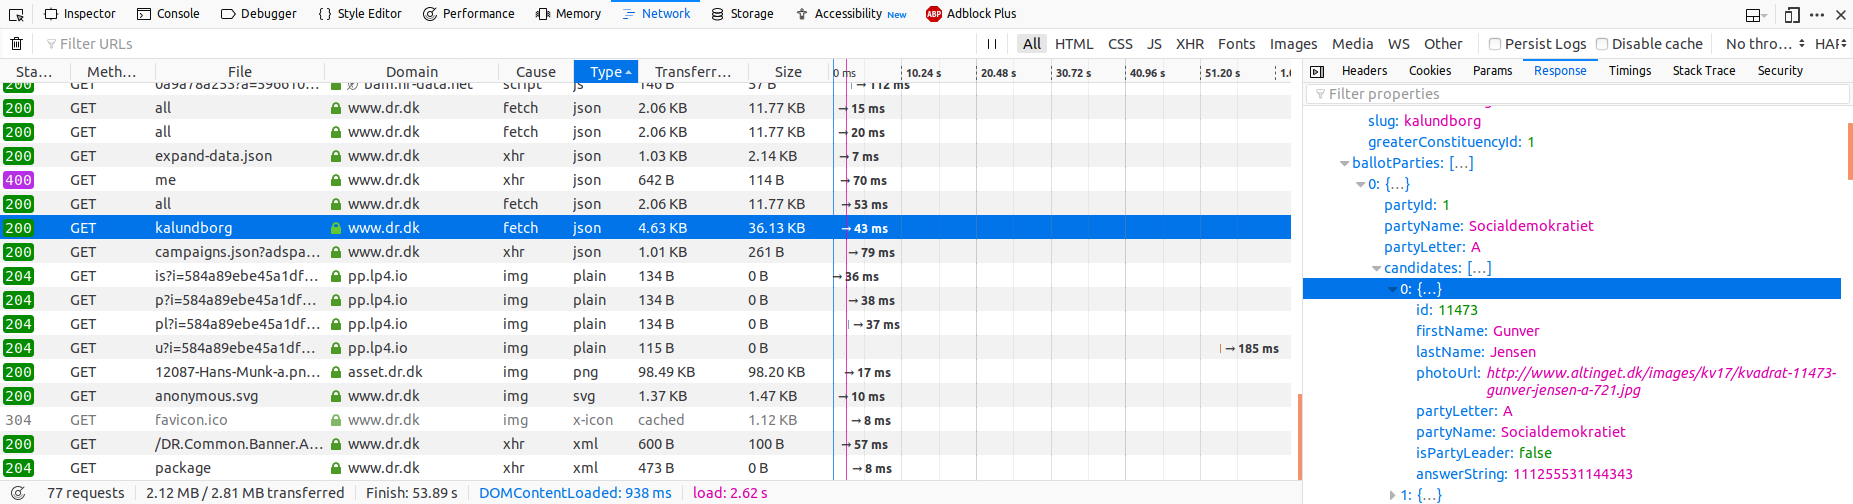
\includegraphics[width=\textwidth]{figs/console.png}
  \end{figure}
\end{frame}

\begin{frame}[fragile]{Opgave 1.4}
  \begin{lstlisting}[language=python]
def hent_kommune_data(kommuneslug):
    base = 'https://www.dr.dk/tjenester/kv17-candidateapi/'
    url = base + f'api/ballot/{kommuneslug}'

    response = requests.get(url)

    if response.ok:
        return response.json()
    else:
        return None
  \end{lstlisting}
\end{frame}

\begin{frame}[fragile]{Opgave 1.5}
  \begin{lstlisting}[language=python, basicstyle=\tiny]
  import pandas as pd

  def rens_kommune_data(kommunejson):
    ballot = kommunejson['ballot']['constituency']
    parties = kommunejson['ballot']['ballotParties']

    _name = ballot['slug']
    _id = ballot['id']

    for party in parties:
        party_candidates = party['candidates']

        for candidate in party_candidates:
            _fname = candidate['firstName']
            _lname = candidate['lastName']

            data = {'id': [_id],
                    'kommune': [_name],
                    'letter': [candidate['partyLetter']],
                    'party': [candidate['partyName']],
                    'name': ['{} {}'.format(_fname, _lname)],
                    'answers': [candidate['answerString']]
                   }
            try:
                df = pd.concat([df, pd.DataFrame(data)])
            except NameError:
                df = pd.DataFrame(data)

    return df.reset_index(drop = True)
  \end{lstlisting}
\end{frame}

\begin{frame}[fragile]{Opgave 1.6}
\begin{lstlisting}[language=python]
from time import sleep

for kom in slugs:
    sleep(2)
    print(kom)
    data = hent_kommune_data(kom)
    clean = rens_kommune_data(data)

    try:
        df = pd.concat([df, pd.DataFrame(clean)])
    except NameError:
        df = pd.DataFrame(clean)
\end{lstlisting}
\end{frame}
\begin{frame}[fragile]{Opgave 1.7}
  \begin{lstlisting}[language=python]
df.reset_index(drop = True)\
  .to_csv('../data/candidates.csv',
          index = False)
  \end{lstlisting}
\end{frame}

\section{Næste gang/tak for i dag}
\begin{frame}[fragile]{Næste gang/tak for i dag}
\begin{itemize}
\item Vi lægger en rettevejledning ud til dagens øvelser på github
\item Vi lægger datasættet op før næste øvelsesgang - \textit{ikke} nødvendigt med hjemmearbejde!
\pause
\item[]
\item[] Næste gang:
\item Samme tid, samme sted, næste fredag.
\item Vi skal lave noget analyse på de data i har scrapet i dag.
\end{itemize}
\end{frame}

\end{document}
